\documentclass[10pt]{article}

\usepackage[latin1]{inputenc}
\usepackage{amsmath, amssymb, amsfonts, amsthm} \usepackage{upgreek} \usepackage{amsthm} \usepackage{fullpage}
\usepackage{graphicx}
\usepackage{cancel}
\usepackage{subfigure}
\usepackage{mathrsfs}
\usepackage{outlines}
\usepackage[font={sf,it}, labelfont={sf,bf}, labelsep=space, belowskip=5pt]{caption}
\usepackage{hyperref}
% \usepackage{minted}
\usepackage{titling}
\usepackage{xifthen}
\usepackage{color}

\usepackage{fancyhdr}
\usepackage[title]{appendix}
\usepackage{float}

\usepackage{siunitx}

\newcommand{\TODO}[1]{\textbf{****** {\bf{[#1]}} ******}}

\usepackage{prettyref}
\newrefformat{sec}{Section~\ref{#1}}
\newrefformat{tbl}{Table~\ref{#1}}
\newrefformat{fig}{Figure~\ref{#1}}
\newrefformat{chp}{Chapter~\ref{#1}}
\newrefformat{eqn}{\eqref{#1}}
\newrefformat{set}{\eqref{#1}}
\newrefformat{alg}{Algorithm~\ref{#1}}
\newrefformat{apx}{Appendix~\ref{#1}}
\newrefformat{prop}{Proposition~\ref{#1}}
\newcommand\pr[1]{\prettyref{#1}}

\usepackage{mathtools}

\DeclareMathOperator{\tr}{tr}
\DeclareMathOperator{\sgn}{sgn}
\DeclareMathOperator{\sinc}{sinc}
\DeclareMathOperator{\rref}{rref}
\DeclareMathOperator{\cof}{cof}
\DeclareMathOperator*{\sym}{sym}
\DeclareMathOperator{\image}{im} % image space of a linear transform

\DeclareMathOperator{\diag}{diag}
\DeclareMathOperator*{\argmax}{argmax}
\DeclareMathOperator*{\argmin}{argmin}
\newcommand{\defeq}{\vcentcolon=}

\renewcommand{\Re}{\operatorname{Re}} \renewcommand{\Im}{\operatorname{Im}}

\providecommand{\norm}[1]{\lVert#1\rVert}
\providecommand{\normlr}[1]{\left\lVert#1\right\rVert}

\providecommand{\tpder}[4]{\frac{\partial^3 #1}{\partial #2 \partial #3 \partial #4}}

\def\jointset{\mathcal{J}}
\def\actjoints{\mathcal{J}'}
\def\rodset{\mathcal{R}}

\renewcommand{\vec}[1]{{\bf #1}}
\def\xflat{\vec{x}^*_\text{2D}}
\def\xdeploy{\vec{x}^*_\text{3D}}
\def\xtgt{\vec{x}_\text{tgt}}

\usepackage{bm}
\def\torques{{\bm \tau}}

\def\R{\mathbb{R}}

\def\normal{{\bm n}}
\def\n{\normal}
\def\a{\vec{a}}
\def\b{\vec{b}}
\def\c{\vec{c}}
\def\d{\vec{d}}
\def\t{\vec{t}}
\def\x{\vec{x}}
\def\X{\vec{X}}
\def\y{\vec{y}}
\def\z{\vec{z}}
\def\u{\vec{u}}
\def\f{\vec{f}}
\def\g{\vec{g}}
% \def\w{\boldsymbol{\omega}}
\def\w{\vec{w}}
\def\wn{\norm{\w}}
\def\p{\vec{p}}
\def\q{\vec{q}}
\def\v{\vec{v}}
\def\e{\vec{e}}
\def\ue{\vec{u}^\e}
\def\fu{\pder{\f}{u}}
\def\fv{\pder{\f}{v}}
\def\strain{\varepsilon}
\def\stress{\sigma}
\def\kb{\kappa \b}
\def\kbi{(\kappa \b)_i}
\def\kn{\bm{\kappa}}
\def\k{\kappa}
\def\R{\, \mathbb{R}}
\def\L{\, \mathcal{L}}
\def\deployAmount{\overline{\alpha}}
\def\deployTgt{\overline{\alpha}^\text{tgt}}

\def\wref{\hat{\w}}

\providecommand{\abs}[1]{\lvert#1\rvert}
\providecommand{\norm}[1]{\lVert#1\rVert}
\providecommand{\normlr}[1]{\left\lVert#1\right\rVert}
\providecommand{\dx}{\, \mathrm{d}x}
\providecommand{\ds}{\, \mathrm{d}s}
\providecommand{\lint}[3]{\int_{#1}^{#2} \! #3 \, \ds}
% \providecommand{\vint}[2]{\int_{#1} \! #2 \, \mathrm{d}x}
% \providecommand{\sint}[2]{\int_{\partial #1} \! #2 \, \mathrm{d}A}
\renewcommand{\div}{\nabla \cdot}
\providecommand{\cross}{\times}
\providecommand{\curl}{\nabla \cross}
\providecommand{\grad}{\nabla}
\providecommand{\laplacian}{\bigtriangleup}
\providecommand{\shape}{\Omega}
\providecommand{\mesh}{\mathcal{M}}
\providecommand{\boundary}{\partial \shape}
\providecommand{\vint}[3][\x]{\int_{#2} \! #3 \, \mathrm{d}#1}
\providecommand{\sint}[3][\x]{\int_{#2} \! #3 \, \mathrm{d}A(#1)}
\providecommand{\pder}[2]{\frac{\partial #1}{\partial #2}}
\providecommand{\spder}[3]{\frac{\partial^2 #1}{\partial #2 \partial #3}}
\providecommand{\spderx}[1]{\frac{\partial^2 #1}{\partial \x^2 }}
\providecommand{\tder}[2]{\frac{\mathrm{d} #1}{\mathrm{d} #2}}
\providecommand{\evalat}[2]{\left.#1\right|_{#2}}
\renewcommand{\vec}[1]{{\bf #1}}

\providecommand{\shapeder}[2]{{\mathrm{d} #1}[#2]}
\providecommand{\matder}[1]{\dot{#1}}

\providecommand{\tderatzero}[2]{\left.\frac{\mathrm{d} #1}{\mathrm{d} #2}\right|_{#2 = 0}}

\providecommand{\compose}{\circ}
\providecommand{\surface}{\Gamma}
\providecommand{\surfacegrad}{\nabla_\surface}
\providecommand{\surfacediv}{\surfacegrad \cdot}
\providecommand{\surfacelaplacian}{\laplacian_\surface}

\providecommand{\epssurface}{{\Gamma_\epsilon}}
\providecommand{\epssurfacegrad}{\nabla_\epssurface}
\providecommand{\epssurfacediv}{\epssurfacegrad \cdot}
\providecommand{\epsnormal}{\normal_\epsilon}
\providecommand{\epsnormalmat}{\tilde{\normal}_\epsilon}
\providecommand{\epsphi}{\phi_\epsilon}
\providecommand{\normalmatder}{\dot{\normal}}
\providecommand{\shapefunc}{{\bm \phi}}

\def\vt{\vec{v}_t}
\def\k{\kappa}

\providecommand\ts[1]{\widehat{\vec{t}^{#1}}}
\providecommand\ds[2]{\widehat{\vec{d}^{#1}_{#2}}}
\providecommand\rd[2]{\underline{\vec{d}^{#1}_{#2}}}
\providecommand\rds[2]{\widehat{\underline{\vec{d}^{#1}_{#2}}}}
\providecommand{\PXport}[1]{P_{\ts{#1}}^{\t^{#1}}}
\providecommand{\ki}[2]{(\k_{#1})_i^{#2}}

\newtheorem{lemma}{Lemma}
\newtheorem{proposition}{Proposition}
\newtheorem{corollary}{Corollary}

\usepackage{mathtools}
\newcases{mycases}{\quad}{%
  \hfil$\m@th\displaystyle{##}$}{$\m@th\displaystyle{##}$\hfil}{\lbrace}{.}
\makeatother

\def\thedate{August 23, 2019}

\newcommand{\documenttitle}{Structural Analysis with Discrete Elastic Rods}

% \allowdisplaybreaks
\pagestyle{fancy}
\headheight 24pt
\headsep    12pt
\lhead{\documenttitle}
\rhead{\thedate}
\fancyfoot[C]{} % hide the default page number at the bottom
\lfoot{}
\rfoot{\thepage}
\renewcommand{\headrulewidth}{0.4pt}
\renewcommand\footrulewidth{0.4pt}

\def\mpa{\si{\mega\pascal} }
\def\mm{\si{\milli\meter} }

\newcommand*{\rom}[1]{\expandafter\@slowromancap\romannumeral #1@}
\newcommand{\RN}[1]{\textup{\uppercase\expandafter{\romannumeral#1}}}

\makeatletter

\setlength{\droptitle}{-50pt}
\title{\documenttitle}
\author{Julian Panetta}
\date{\thedate}

% BEGIN DOCUMENT
\begin{document}
\maketitle

This document details how the discrete elastic rods model can be used to
evaluate important structural aspects of a deployed gridshell such as the
internal stresses in its beams and the forces acting on its bolts.
We separately consider internal stresses due to stretching, bending, and twisting.
The stretching and bending stresses can be naturally superimposed because they
both take the form of a ``$z$-stress'' (i.e., tensile/compressive forces oriented
along the tangential direction). We will see that twisting stresses are slightly different,
and note that our analysis cannot capture the interplay of bending and twisting
stresses with complete accuracy.

A note on units: we prefer \si{\newton} for force, \mm for length, and
\mpa for stress. However no units are actually specified in the code or
equations, so any compatible system of units can be chosen. For example, one
could instead use \si{\newton}, \si{\meter}, and \si{\pascal}.

\section{Stretching Stress}
The simplest energy term to analyze is stretching, as the strain and stress are just
the familiar $1$D quantities $\frac{\Delta l}{l}$ and $E \frac{\Delta l}{l}$,
where $l$ is the length of a small segment of rod and $E$ is the Young's modulus.
This quantity lives most naturally on the edges, but it could be averaged onto
the vertices if desired.

\section{Bending Stress}
When a segment of rod is bent, it causes stretching in one ``half'' of the
cross-section and compression in the other. We consider a cross-section $\Omega$
with a center of mass $\c$. We bend the rod segment so that its centerline
centerline has the \emph{curvature normal} vector $\kn$, arriving at the
following configuration:
\begin{figure}[h]
    \centering
    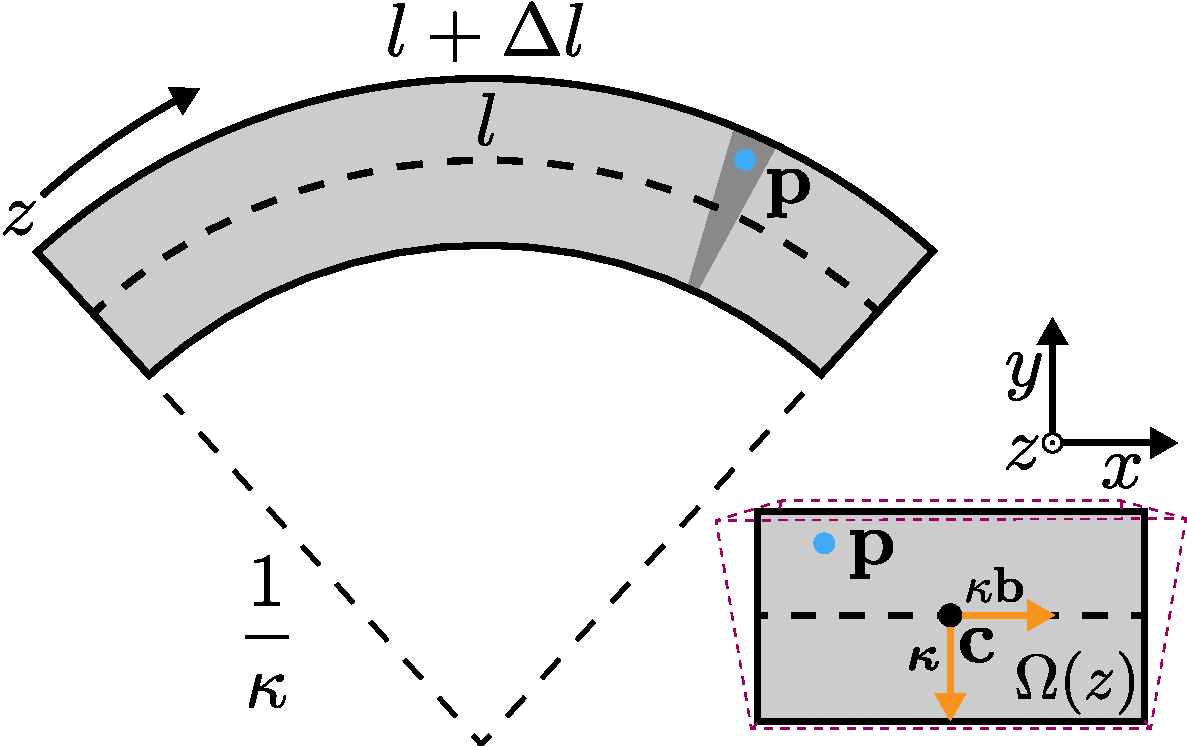
\includegraphics[width=0.5\textwidth]{BendingFigure.pdf}
    \caption{Geometry of a bent rod.}
    \label{fig:bent_rod}
\end{figure}

\noindent
The dashed line parallel to the curvature binormal $\kb$ and passing through the
center of mass indicates the neutral surface, which experiences no strain under
this bending deformation. This neutral surface divides $\Omega$ into two
halves: the half pointed to by $\kn$ which experiences a compressive
$z$ strain, and the other half which experiences a tensile $z$ strain.

Studying the deformation, we see that at a particular signed height $h$ ``above'' (in the opposite direction of $\kn$) the
neutral surface, the deformed length is $l + \Delta l = \frac{l}{1 / \kappa} \left(\frac{1}{\kappa} + h\right) = l + h \kappa \l$,
indicating a $z$ strain of $\frac{\Delta l}{l} = h \kappa$.
The $z$ strain at some point $\p \in \Omega(z)$ can be therefore written as
$\strain_{zz} = -\kn \cdot (\p - \c) = \kn \cdot (\c - \p)$, and under our isotropic linear material
model, the stress is $\stress_{zz} = E \kn \cdot (\c - \p)$.

For engineering applications, we want to know the maximum and minimum principal stresses occurring in each
cross-section of the beam. The formula for $\stress_{zz}$ is linear in $\p$ and therefore must
achieve its maximum and minimum on the boundary of $\Omega(z)$. However the
particular boundary location of the maximum stress depends on the direction of
$\kn$, and for general cross-section geometries we will need to check every
boundary point of the mesh as the boundary may have concave regions.

In the discrete elastic rods model, we discretize the curvature quantities on
the vertices and store the material frames/cross sections on the edges. So, to
estimate the principal stresses, we will need to transfer quantities between
vertices and edges. We compute two versions of the maximum/minimum principal
stresses at a vertex, one using the material frame from the incoming edge and
another using the frame from the outgoing edge. We then take a length-weighted
average of these quantities to define the vertex stresses. The resulting vertex
stress expressions are:
\begin{align*}
\stress_{zz}^\text{max} &=
    \frac{1}{2 \overline{l}_i} \left[
        \frac{\overline{l}^{i - 1}}{\overline{l}_{i}} E^{i - 1} \left(\max_{\p \in \Omega^{i - 1}} \begin{bmatrix} \ki{1}{i - 1} \\ \ki{2}{i - 1} \end{bmatrix} \cdot (\c - \p) \right) +
        \frac{\overline{l}^{i    }}{\overline{l}_{i}} E^{i    } \left(\max_{\p \in \Omega^{i    }} \begin{bmatrix} \ki{1}{i    } \\ \ki{2}{i    } \end{bmatrix} \cdot (\c - \p) \right)
    \right] \\
\stress_{zz}^\text{min} &=
    \frac{1}{2 \overline{l}_i} \left[
        \frac{\overline{l}^{i - 1}}{\overline{l}_{i}} E^{i - 1} \left(\min_{\p \in \Omega^{i - 1}} \begin{bmatrix} \ki{1}{i - 1} \\ \ki{2}{i - 1} \end{bmatrix} \cdot (\c - \p) \right) +
        \frac{\overline{l}^{i    }}{\overline{l}_{i}} E^{i    } \left(\min_{\p \in \Omega^{i    }} \begin{bmatrix} \ki{1}{i    } \\ \ki{2}{i    } \end{bmatrix} \cdot (\c - \p) \right)
    \right].
\end{align*}
The multiplication by $\frac{\overline{l}^j}{\overline{l}_i}$ converts the integrated curvature normal (integrated over
a vertex Voronoi region) into a pointwise value and then integrates it over half of the associated incident edge to perform
the weighted average.
Note that $\ki{a}{j}$ is the curvature normal vector expressed in the material
frame for edge $j$, so the diagram in \pr{fig:bent_rod} applies (although $\kn$
can be rotated arbitrarily depending on the bending axis!). Also, in our
implementation, the cross-section's center of mass is translated to the origin,
so $\c$ vanishes from the formula.

\section{Twisting Stress}
Under an imposed rate of twist $\tau_i = \frac{m_i - \overline{m}_i}{\overline{l}_i}$, a cross-section will experience the stress distribution:
$$
\sigma(x, y) = \mu \tau_i \begin{bmatrix}
    0 & 0 & \pder{\psi}{x} - y \\
    0 & 0 & \pder{\psi}{y} + x \\
    \pder{\psi}{x} - y & \pder{\psi}{y} + x & 0
\end{bmatrix},
$$
where $\psi$ is the out-of-plane warping function found as the solution to the Laplace equation
$\bigtriangleup \psi = 0$ in $\Omega$ with Neumann boundary conditions ${\bf n} \cdot \nabla \psi = {\bf n} \cdot \begin{pmatrix} y \\ -x \end{pmatrix}$ on $\partial \Omega$
when computing the twisting stiffness.
This stress tensor has two nonzero eigenvalues, $\sigma_{z*} \defeq \pm \left\|\grad \psi +
\begin{bmatrix} - y \\ x \end{bmatrix}\right\|$, indicating the principal
tensile and compressive stresses associated with the torsional shearing. We
choose to report only the positive eigenvalue.

As with bending stresses, because the cross-sections live on the edges
and the twists on the vertices, we must perform an averaging procedure. We
compute a weighted average of the maximum shearing stress induced by a vertex's
twist as measured in the incoming and outgoing edges:
$$
\stress_\tau = \tau_i \frac{S^{i - 1} \overline{l}^{i - 1} + S^i \overline{l}^i}{2 \overline{l}_i},
\quad
S^j \defeq \mu^{j}\max_{\p \in \Omega^j} \left\|\grad \psi + R^{{90}^\circ}(\p - \c) \right\|.
$$
$S^j$ is not load-dependent and can be pre-computed for each cross-section appearing in the design when computing the
material parameters.
Finally, we note that the ``twisting'' stress $\stress_\tau$ is in the form of a shear traction acting on the cross-section.

\section{Rivet Axial/Shearing Forces}
We can compute the forces acting on the rivets/bolts binding the rods by summing the elastic forces over all the $A$ rods while
omitting the $B$ rods. The components of this (partial) elastic energy gradient that correspond to the joints'
degrees of freedom no longer vanish and inform us of the generalized
forces applied by the $A$ rods on the joint geometry. These will be balanced
by equal and opposite generalized forces from the $B$ rods. This force vector is computed
by \texttt{RodLinkage::rivetForces}.

There are three types of joint variables leading to three types of generalized forces. The (negated) gradient with respect to the joint
position tells us the net force acting on the joint's center of mass. The (negated) gradient with respect to the orientation variables
$\omega$ tells us the net torques acting around the global coordinate axes at the joint's center of mass (in units \si{\newton \milli\meter}).
Finally the gradient with respect to the two length variables relate to tensile forces acting on the rods, but these forces should
be in balance (i.e., these components of the gradient should remain zero even when we drop the contributions from $B$ rods).

The net force acting on the joint can be decomposed into a component along the joint normal that applies a tensile/compressive load
to the bolt and a component perpendicular to the normal that attempts to shear the bolt. The net torque acting on the joint's frame
also introduces shearing forces on the joint.

\section{Tutorial}
A Jupyter notebook demonstrating these features is available in \texttt{python/examples/StructuralAnalysis.ipynb} of the
\href{https://github.com/jpanetta/ElasticRods}{ElasticRods} codebase.

\end{document}
